% http://www.math.umbc.edu/~rouben/beamer/

\documentclass[12pt]{beamer}
\usetheme{Copenhagen}

\usefonttheme{structurebold} 

\setbeamertemplate{blocks}[rounded][shadow=true] 
% itemize levels
\setbeamertemplate{itemize item}{\scriptsize\raise1.25pt\hbox{\donotcoloroutermaths$\blacksquare$}}
\setbeamertemplate{itemize subitem}{\tiny\raise1.5pt\hbox{\donotcoloroutermaths$\blacktriangleright$}}
%\setbeamertemplate{itemize subitem}{--}
\setbeamertemplate{itemize subsubitem}{\tiny\raise1.5pt\hbox{\donotcoloroutermaths$\star$}}
% enumerate levels
\setbeamertemplate{enumerate item}{\insertenumlabel.}
\setbeamertemplate{enumerate subitem}{\insertenumlabel.\insertsubenumlabel}
\setbeamertemplate{enumerate subsubitem}{\insertenumlabel.\insertsubenumlabel.\insertsubsubenumlabel}
\setbeamertemplate{enumerate mini template}{\insertenumlabel}

\setbeamertemplate{navigation symbols}{}
%\setbeamertemplate{items}[ball]
\setbeamersize{text margin left=6mm, text margin right=6mm}


%\useoutertheme{infolines}
\author{Markus Schordan and Adrian Prantl} 
\institute{FH Technikum Wien, Austria\\and\\Lawrence Livermore National Laboratory, CA, USA} 

% compatibility defs for commands used in original prosper files
\newcommand{\ptsize}[1]{\fontsize{#1}{12}\selectfont } % we ignore this command

% defs for ignoring different parts
\newcommand{\optimization}[1]{#1} % we ignore optimizations with {} (otherwise use {#1}.
\newcommand{\advancedtopic}[1]{#1} % we ignore advanced topics with {} (otherwise use {#1}.
\newcommand{\ignore}[1]{} % we ignore some slides

\usepackage{color} % load color package
%\definecolor{<color_name>}{<color model>}{<values>}

\usepackage{latexsym}
\usepackage{amssymb}   
\usepackage{epsfig}
%\usepackage{psfig}
%\usepackage{epsf}
\usepackage{graphicx}

\usepackage[utf8]{inputenc}
\usepackage[english]{babel}
\usepackage{cite}
%\usepackage[cmex10]{amsmath}   % for \split etc.
%\usepackage[usenames]{color}
\usepackage{graphicx}
%\usepackage{array}  % for tables
\usepackage{mdwtab}
\usepackage{rotating}  % for tables
\usepackage{multicol}  % for tables
\usepackage{multirow}  % for tables
\usepackage{verbatim}
\usepackage{algorithmicx}
\usepackage{algorithm2e}
%\usepackage[ruled]{algorithm}
%\usepackage{algpseudocode}
\usepackage{picture}
\usepackage[final]{pdfpages}
\usepackage{setspace}
\usepackage{alltt} % for fixed-width font sourcecode figures
\usepackage{tikz}
\usepackage{listings}

% making bitmap graphics in PDF look good
% ps2pdf -dAutoFilterColorImages=false -dColorImageFilter=/FlateEncode

% transitions: Split Blinds Box Wipe Dissolve Glitter Replace (default) 
% begin{slide}[transition]{title}

% syntax for defining colors; color models can be, rgb, cmyk, gray;
% values are comma separated decimal values
% color names can be any logical name you might assign for a color

% eg:
% HEX: 006666 -> range[0,1] -> 
\definecolor{lavender}{rgb}{.0,.32,.32}
\definecolor{algomarkcolor}{rgb}{.82,.82,.42}
\definecolor{black}{rgb}{.0,.0,.0}
\definecolor{red}{rgb}{1.0,.0,.0}
\definecolor{green}{rgb}{.1,0.6,.1}
\definecolor{blue}{rgb}{.0,.0,1.0}
\definecolor{lightblue}{rgb}{.3,.3,0.8}
%
%\definecolor{gray10}{gray}{.9} % 10% gray
%
% Usage:
%
%\textcolor{lavender}{text material to appear in lavender color}
%
%or 
%
%\color{lavender} Material to appear in color .... \normalcolor
%
%or you might define environments which would start and end the
%particular color you want.
%
%Useful documentation:
%
%* grfguide.ps(.gz), which is available in any standard TeX distribution.
%
%* TUGIndia on-line tutorial which describes color table available at:
%  http://www.tug.org.in/tutorials.html 
%* proper tutorial
%  http://www.math.umbc.edu/~rouben/prosper

% how to include graphics (e.g.: 3 pics side-by-side):
%\bigskip
%\begin{center}
%    \includegraphics[height=35mm]{ns-2d-u.eps}
%    \includegraphics[height=35mm]{ns-2d-v.eps}
%    \includegraphics[height=35mm]{ns-2d-p.eps}
%\end{center}

% LOGO: \Logo{\umbclogo}
%       \Logo{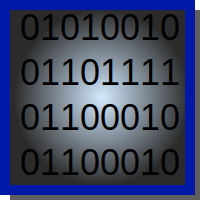
\includegraphics{logo.eps}}
%       \Logo(x,y){someobject}.

% \hyperlink{mytarget}{Click here} to go to the target slide.
% \hypertarget{mytarget}{}
% in acrobat reader: use <CTRL>+<LEFT ARROW> to return to a source-page.

% \href{run:movie.mpg}{Start Movie}

% set default font size
% \ptsize{n}, with in {8, 9, 10, 11, 12, *14*, 17}
\ptsize{12}

%\input{~/diss/thesis/formalisms}

% mehrspaltiges layout
% \begin{minipage}[t]{0.7\textwidth}
% linke seite
% \end{minipage}
% % KEINE LEERZEILE (sonst minipages untereinander)
% \begin{minipage}[t]{0.7\textwidth}
% rechte seite
% \end{minipage}

% selbstdefinierte kopf und fuSzeilen
% package fancyhdr


%\leftFOOT{Markus Schordan}
%\rightFOOT{RIGHT}
%\centerFOOT{\today}

%fake
%\newcommand{\textsc}[1]{} % 
